\documentclass[a4paper,kul]{kulakarticle} %options: kul or kulak (default)

\usepackage[utf8]{inputenc}
\usepackage[english]{babel}
\usepackage{graphicx}
\usepackage{subcaption}
\newlength{\twosubht}
\newsavebox{\twosubbox}
\graphicspath{{../Figures/}{../Matlab/}{/}}
\usepackage[outdir=./]{epstopdf}

\usepackage{amsmath}
\usepackage{amsthm}
\usepackage{amssymb}
\usepackage{gensymb}
\setcounter{MaxMatrixCols}{21}

\usepackage{etoolbox,refcount}
\usepackage{multicol}

\newcounter{countitems}
\newcounter{nextitemizecount}
\newcommand{\setupcountitems}{%
	\stepcounter{nextitemizecount}%
	\setcounter{countitems}{0}%
	\preto\item{\stepcounter{countitems}}%
}
\makeatletter
\newcommand{\computecountitems}{%
	\edef\@currentlabel{\number\c@countitems}%
	\label{countitems@\number\numexpr\value{nextitemizecount}-1\relax}%
}
\newcommand{\nextitemizecount}{%
	\getrefnumber{countitems@\number\c@nextitemizecount}%
}
\newcommand{\previtemizecount}{%
	\getrefnumber{countitems@\number\numexpr\value{nextitemizecount}-1\relax}%
}
\makeatother    
\newenvironment{AutoMultiColItemize}{%
	\ifnumcomp{\nextitemizecount}{>}{3}{\begin{multicols}{2}}{}%
		\setupcountitems\begin{itemize}}%
		{\end{itemize}%
		\unskip\computecountitems\ifnumcomp{\previtemizecount}{>}{3}{\end{multicols}}{}}

\usepackage{pdflscape}

\date{Academic year 2021 -- 2022}
\address{
  Faculty of Engineering Science \\
  Department of Mechanical Engineering \\
  Control theory \texttt{[H04X3a]}}
\title{Report Assignment 2: Velocity control of the cart}
\author{Matthias Derez, Toon Servaes}


\begin{document}

\maketitle
\section{Introduction}
In this report, two velocity controllers for DC motors are designed, using frequency respons methods. The main criterion states that the velocity controller yieldaangeziens a zero steady-state error on a constant velocity reference. 
\section{Design of the controller}
\subsection{Type of the controller}
To satisfy the criterion of zero steady-state error, multiple controllers can be used. A PI, PID and feedforward controller can all yield a zero steady-state error. The feedforward controller can be especially usefull for tracking. However, as the controller must yield a zero steady-state error on a constant velocity reference and deal with errors caused by disturbances, the feedforward controller will not be used. Since a large bandwidth yields a fast responding system, a high bandwidth seems advantaegous. If the bandwidth is too high though, the high frequency noise has more influence. A trade-off between the two has to be made. Generally the sampling frequency has to be at least 10-20 times larger than bandwidth (\underline{REFERENTIE C8 S82}). In this report, the bandwidth will be approximated by the crossover frequency $\omega_c$. Because of teh aforementioned reasons and because of simplicity the PI controller is chosen, as the extra bandwith delivered by the D (or lead) part in the PID controller is unnecessary.  
\subsection{Design parameters}
To properly execute the design, some design parameters must be determined. The parameters that can be chosen free are the phase margin (PM) and the extra margin $d\phi$ to compensate for the phase lag. Using these, the new cross over frequency $\omega_c$, the integration time $T_i$, the gain and the gain margin (GM) of the controller can be calculated. 
%Firstly, we write down the used values and equations, later on additional information will be given on why these values are chosen and the relations between the variables.% 



\subsubsection{Phase margin}
The design value of the PM lies between 40\degree to 50\degree. We know that by increasing the PM, the damping $\zeta$ (REFERENCE C7 S26) and $T_i$ will increase. The peak value in the closed loop step response $M_p$ (REFERENCE C7 S27) and the new cross over frequency $\omega_c$ will decrease. The increase in $\zeta$ causes the respons of the signal to be slower, but have less oscillations. Since the value of $\zeta$ is still below the value of critical damping of $\zeta = 0.7$, the increase is in general advantageous for the transient respons. The decrease of $\omega_c$ is helps to keep the cross over frequency 10-20 times lower than the sampling frequency and reduces the influence of high frequency noise. However, $\omega_c \gg \frac{1}{T_i}$ is necessary to lower the influence of the phase lag introduced by the PI controller. Luckily by increasing the PM, $\frac{1}{T_i}$ decreases (REFERENTIE FORMULE Ti) and thus the fact that $\omega_c$ reduces, is partly compensated by the decrease in $\frac{1}{T_i}$. Additionally, if $T_i$ decreases there is more/faster integrating action. The decrease in overshoot $M_p$ improves the transient respons. By processing the data in Matlab, it becomes clear that by increasing the PM, the GM increases and the transient error decreases (TONEN VIA MATLAB?). For these reasons, the PM is chosen to be equal to 50\degree. 

\subsubsection{Extra margin to compensate for the phase lag}
	As the PI controller has a negative phase, an extra margin $d\phi$ on the PM has to be included to calculate the new cross over frequency $\omega_c$. The chosen margin can vary from 10\degree to 15\degree. By choosing a higher value, $T_i$ decreases, ass is shown in Equation \ref{eq: Ti}. This helps lower the influence of the phase lag. As you anticipate more influence of the phase lag, the $\omega_c$ will decrease, but since the value is quite close to the maximum value of $\frac{f_s}{10}$ this is not that disadvantageous. By using different values and calculating the stepresponse on the closed loop system in Matlab, it is clear the total added transient error decreases when the extra margin is increased. $d\phi = 15\degree$ is chosen. 

\subsubsection{Design procedure}
Now the PM and the extra margin on the PM are chosen, the frequency where the uncompensated open loop system has a phase $\phi = -180\degree + PM + d\phi$ can be determined. This is the new cross over frequency $\omega_c$. Using this result, $T_i$ can be calculated using Equation \ref{eq: Ti}. 

\begin{equation}
	\label{eq: Ti}
	T_i = \frac{\tan(90\degree - d\phi)}{\omega_c}
\end{equation} 
The transfer function of the PI controller can be written as:
\begin{equation}
	\label{eq: TF PI}
	D(s) = \frac{K}{s}(s+\frac{1}{T_i})
\end{equation}
The gain K can be determined, stating that the gain of the compensated system at $\omega_c$ indeed equals 1:
\begin{equation}
	|G(j\omega_c)D(j\omega_c)| = 1
\end{equation}
The gain margin is a measure for stability and reduces resonance. The design value is $GM \approx 2$. The values obtained from these calculations can be found in Table \ref{tab:values}. 

\begin{table}[htp!]
	
	\centering
	
	\begin{tabular}{|l|l|}
		\hline
		Parameter                & Value                         \\ \hline
		GM                       & 1.8132                        \\
		PM                       & 49.2538\degree \\
		$\omega_c$ & 56.0686 rad/s                 \\
		$T_i $                    & 0.0665 s                      \\
		$\frac{1}{T_i}$                    & 15.0264 s                      \\
		$d\phi$             & 15\degree      \\
		gain K 	 		& 1.2518 \\ \hline
	\end{tabular}
	\caption{Design parameters and their calculated values}
	\label{tab:values}
\end{table}
As can be seen in Table \ref{tab:values}, however the difference is quite small and the system shows no sign of instabilities, the value is acceptable. $\frac{1}{T_i}$ is not that much smaller than $\omega_c$, but the influence of the extra phase lag on the other parameters is acceptable. In Figure \ref{fig:bodeplotopenloop} the bodeplots of the different open loop systems are shown and in Figure \ref{fig:bodeplotcl} the bodeplot of the closed loop system is shown. 


OP FIGUUR NOG DINGEN AANDUIDEN
\begin{figure}[htp!]
	\centering
	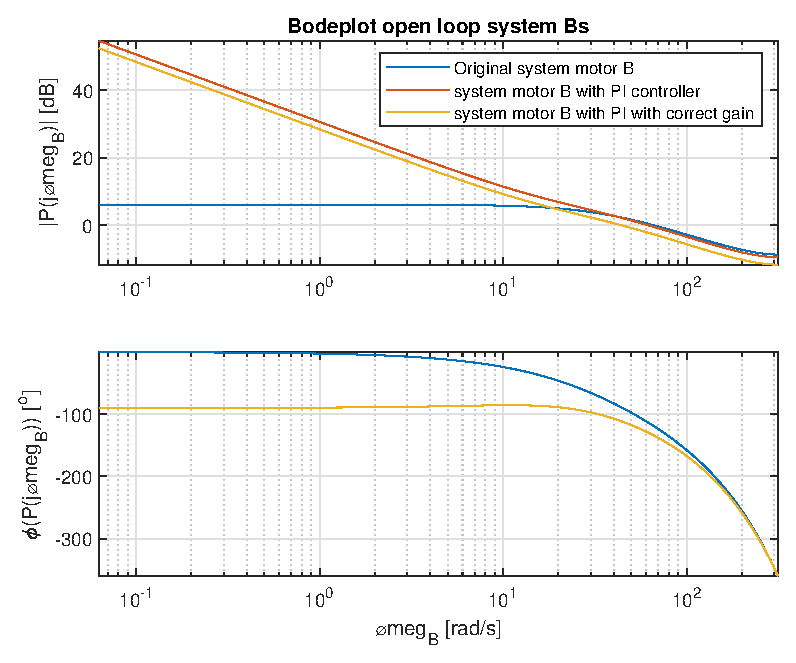
\includegraphics[width=0.6\linewidth]{bodeplot_openloop.eps}
	\caption{Bodeplot of the different open loop systems}
	\label{fig:bodeplotopenloop}
\end{figure}

\begin{figure}[htp!]
	\centering
	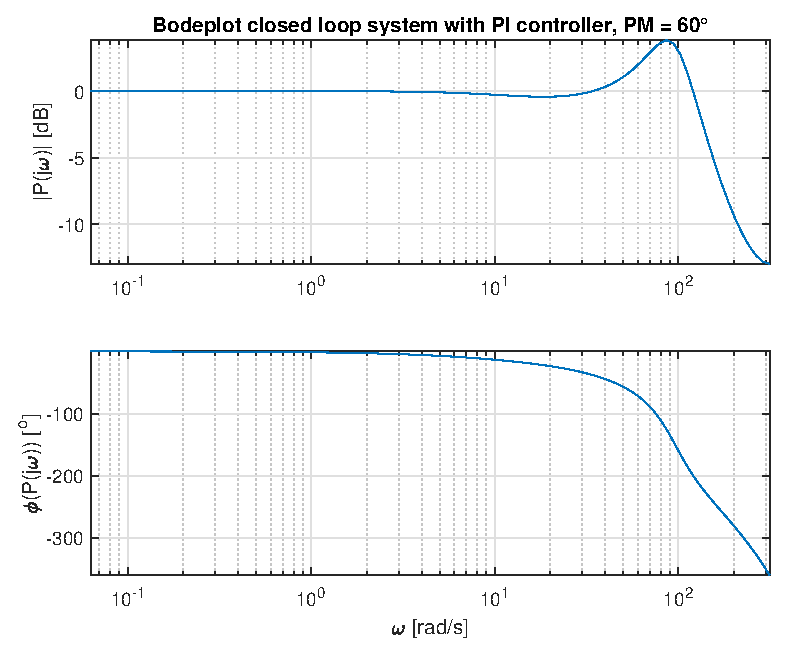
\includegraphics[width=0.6\linewidth]{bodeplot_cl.eps}
	\caption{Bodeplot of the closed loop system with PI controller}
	\label{fig:bodeplotcl}
\end{figure}




\subsection{Limitations on bandwidth}


\section{Validation of the controller}




\end{document}